\documentclass[journal, a4paper]{IEEEtran}
\usepackage{weva}
% \usepackage{amsmath}
\usepackage{graphicx}

% some very useful LaTeX packages include:

%\usepackage{cite}      % Written by Donald Arseneau
                        % V1.6 and later of IEEEtran pre-defines the format
                        % of the cite.sty package \cite{} output to follow
                        % that of IEEE. Loading the cite package will
                        % result in citation numbers being automatically
                        % sorted and properly "ranged". i.e.,
                        % [1], [9], [2], [7], [5], [6]
                        % (without using cite.sty)
                        % will become:
                        % [1], [2], [5]--[7], [9] (using cite.sty)
                        % cite.sty's \cite will automatically add leading
                        % space, if needed. Use cite.sty's noadjust option
                        % (cite.sty V3.8 and later) if you want to turn this
                        % off. cite.sty is already installed on most LaTeX
                        % systems. The latest version can be obtained at:
                        % http://www.ctan.org/tex-archive/macros/latex/contrib/supported/cite/

\usepackage{graphicx}   % Written by David Carlisle and Sebastian Rahtz
                        % Required if you want graphics, photos, etc.
                        % graphicx.sty is already installed on most LaTeX
                        % systems. The latest version and documentation can
                        % be obtained at:
                        % http://www.ctan.org/tex-archive/macros/latex/required/graphics/
                        % Another good source of documentation is "Using
                        % Imported Graphics in LaTeX2e" by Keith Reckdahl
                        % which can be found as esplatex.ps and epslatex.pdf
                        % at: http://www.ctan.org/tex-archive/info/

%\usepackage{psfrag}    % Written by Craig Barratt, Michael C. Grant,
                        % and David Carlisle
                        % This package allows you to substitute LaTeX
                        % commands for text in imported EPS graphic files.
                        % In this way, LaTeX symbols can be placed into
                        % graphics that have been generated by other
                        % applications. You must use latex->dvips->ps2pdf
                        % workflow (not direct pdf output from pdflatex) if
                        % you wish to use this capability because it works
                        % via some PostScript tricks. Alternatively, the
                        % graphics could be processed as separate files via
                        % psfrag and dvips, then converted to PDF for
                        % inclusion in the main file which uses pdflatex.
                        % Docs are in "The PSfrag System" by Michael C. Grant
                        % and David Carlisle. There is also some information
                        % about using psfrag in "Using Imported Graphics in
                        % LaTeX2e" by Keith Reckdahl which documents the
                        % graphicx package (see above). The psfrag package
                        % and documentation can be obtained at:
                        % http://www.ctan.org/tex-archive/macros/latex/contrib/supported/psfrag/

%\usepackage{subfigure} % Written by Steven Douglas Cochran
                        % This package makes it easy to put subfigures
                        % in your figures. i.e., "figure 1a and 1b"
                        % Docs are in "Using Imported Graphics in LaTeX2e"
                        % by Keith Reckdahl which also documents the graphicx
                        % package (see above). subfigure.sty is already
                        % installed on most LaTeX systems. The latest version
                        % and documentation can be obtained at:
                        % http://www.ctan.org/tex-archive/macros/latex/contrib/supported/subfigure/

\usepackage{url}        % Written by Donald Arseneau
                        % Provides better support for handling and breaking
                        % URLs. url.sty is already installed on most LaTeX
                        % systems. The latest version can be obtained at:
                        % http://www.ctan.org/tex-archive/macros/latex/contrib/other/misc/
                        % Read the url.sty source comments for usage information.

%\usepackage{stfloats}  % Written by Sigitas Tolusis
                        % Gives LaTeX2e the ability to do double column
                        % floats at the bottom of the page as well as the top.
                        % (e.g., "\begin{figure*}[!b]" is not normally
                        % possible in LaTeX2e). This is an invasive package
                        % which rewrites many portions of the LaTeX2e output
                        % routines. It may not work with other packages that
                        % modify the LaTeX2e output routine and/or with other
                        % versions of LaTeX. The latest version and
                        % documentation can be obtained at:
                        % http://www.ctan.org/tex-archive/macros/latex/contrib/supported/sttools/
                        % Documentation is contained in the stfloats.sty
                        % comments as well as in the presfull.pdf file.
                        % Do not use the stfloats baselinefloat ability as
                        % IEEE does not allow \baselineskip to stretch.
                        % Authors submitting work to the IEEE should note
                        % that IEEE rarely uses double column equations and
                        % that authors should try to avoid such use.
                        % Do not be tempted to use the cuted.sty or
                        % midfloat.sty package (by the same author) as IEEE
                        % does not format its papers in such ways.

\usepackage{amsmath}    % From the American Mathematical Society
                        % A popular package that provides many helpful commands
                        % for dealing with mathematics. Note that the AMSmath
                        % package sets \interdisplaylinepenalty to 10000 thus
                        % preventing page breaks from occurring within multiline
                        % equations. Use:
%\interdisplaylinepenalty=2500
                        % after loading amsmath to restore such page breaks
                        % as IEEEtran.cls normally does. amsmath.sty is already
                        % installed on most LaTeX systems. The latest version
                        % and documentation can be obtained at:
                        % http://www.ctan.org/tex-archive/macros/latex/required/amslatex/math/



% Other popular packages for formatting tables and equations include:

%\usepackage{array}
% Frank Mittelbach's and David Carlisle's array.sty which improves the
% LaTeX2e array and tabular environments to provide better appearances and
% additional user controls. array.sty is already installed on most systems.
% The latest version and documentation can be obtained at:
% http://www.ctan.org/tex-archive/macros/latex/required/tools/

% V1.6 of IEEEtran contains the IEEEeqnarray family of commands that can
% be used to generate multiline equations as well as matrices, tables, etc.

% Also of notable interest:
% Scott Pakin's eqparbox package for creating (automatically sized) equal
% width boxes. Available:
% http://www.ctan.org/tex-archive/macros/latex/contrib/supported/eqparbox/

% *** Do not adjust lengths that control margins, column widths, etc. ***
% *** Do not use packages that alter fonts (such as pslatex).         ***
% There should be no need to do such things with IEEEtran.cls V1.6 and later.

% Definition of \maketitle
\makeatletter         
\def\@maketitle{
\begin{center}
{\Huge \@title }\\[4ex] 
{\Large  \@author}\\[4ex] 
\end{center}}
\makeatother

% Your document starts here!
\begin{document}

% Define document title and author
\title{FACE {\vspace*{0.20cm}
\includegraphics[width = 7.9mm]{io.png}} FACE \\ \weva{\large{the paintings have eyes}}}
\author{Skander \textbf{Hajri} - Licia \textbf{Tomaselli} - Costanza \textbf{Volpini}}
\markboth{EPFL - Media & Design Lab - Experience Design CS-489}{}
\maketitle

% Write abstract here
\begin{abstract} 
% ALL
We intend to analyse and record feelings and emotions in visitors in front of various paintings and investigate the way they look at artworks. The aim is to set a specific path, museum design and succession of depictions based on a precise sequence of feelings that the viewer or even the organiser of the exhibition wants to evoke.
\end{abstract}

\section{State of art}
\PARstart{R}{everse} your perspective: for once the artwork will look at you like you’re a work of art. Create your own path following your emotions, making your experience in the museum unique. \textit{Be the curator of your own emotions!}
You should not worry anymore about a default museum path. Do you feel a bit sad and you desire to express this feeling during your visit? We have realized a software to handle your museum stay. For our research we have chosen one particular exhibition (Liu Bolin - Le Théâtre des apparences) because his work is not too well known to interfere with the recording of visitors’ impressions and it’s at the same time various (in terms of atmosphere of the work curious for most of the visitors and unconventional). We believe that our project could potentially help visitors to be identified himself more with the artist of the exhibition.

% Each section begins with a \section{title} command
\section{Introduction}
% ALL
\PARstart{F}{ace to face} is a project realized in context of the master course Experience Design, tutored by the professour Jeffrey Huang and Immanuel Koh. The experiment was conducted on a sample of 10 people. We have tried to find peers people with different backgrounds (see graph \ref{fig:sample}).

\begin{figure}[h]
    \centering
    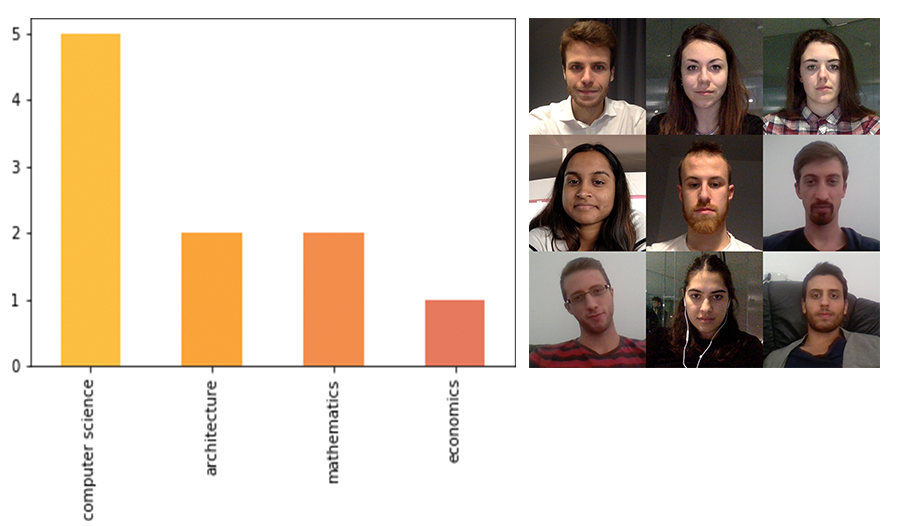
\includegraphics[width=0.47\textwidth]{samplesample.png}
    \caption{Sample analyzed. On the right: 9 of the 10 people analyzed.}
    \label{fig:sample}
\end{figure}


In Section \ref{sec:experiment} we have described the structure of the process to collect our data.
%TODO: add

\section{Experiment} \label{sec:experiment}
\PARstart{T}{o} run the experiment we have implemented a Flask web application. The sample did not know the goal of our experiment, we asked him/her to sit in front of the computer and to watch a sequence of artworks for 2/3 minutes. The sequence of painting should resemble a possible museum path, it is generated randomly for each person to avoid the possibility that an artwork could potentially affected the emotion of the following ones. Each artwork is showed for 6 seconds during which the web camera of the computer records 4 pictures (each one every 1.5 seconds) to detect the emotion trend of an artwork (see Fig. \ref{fig:time}). 
\begin{figure}[h]
    \centering
    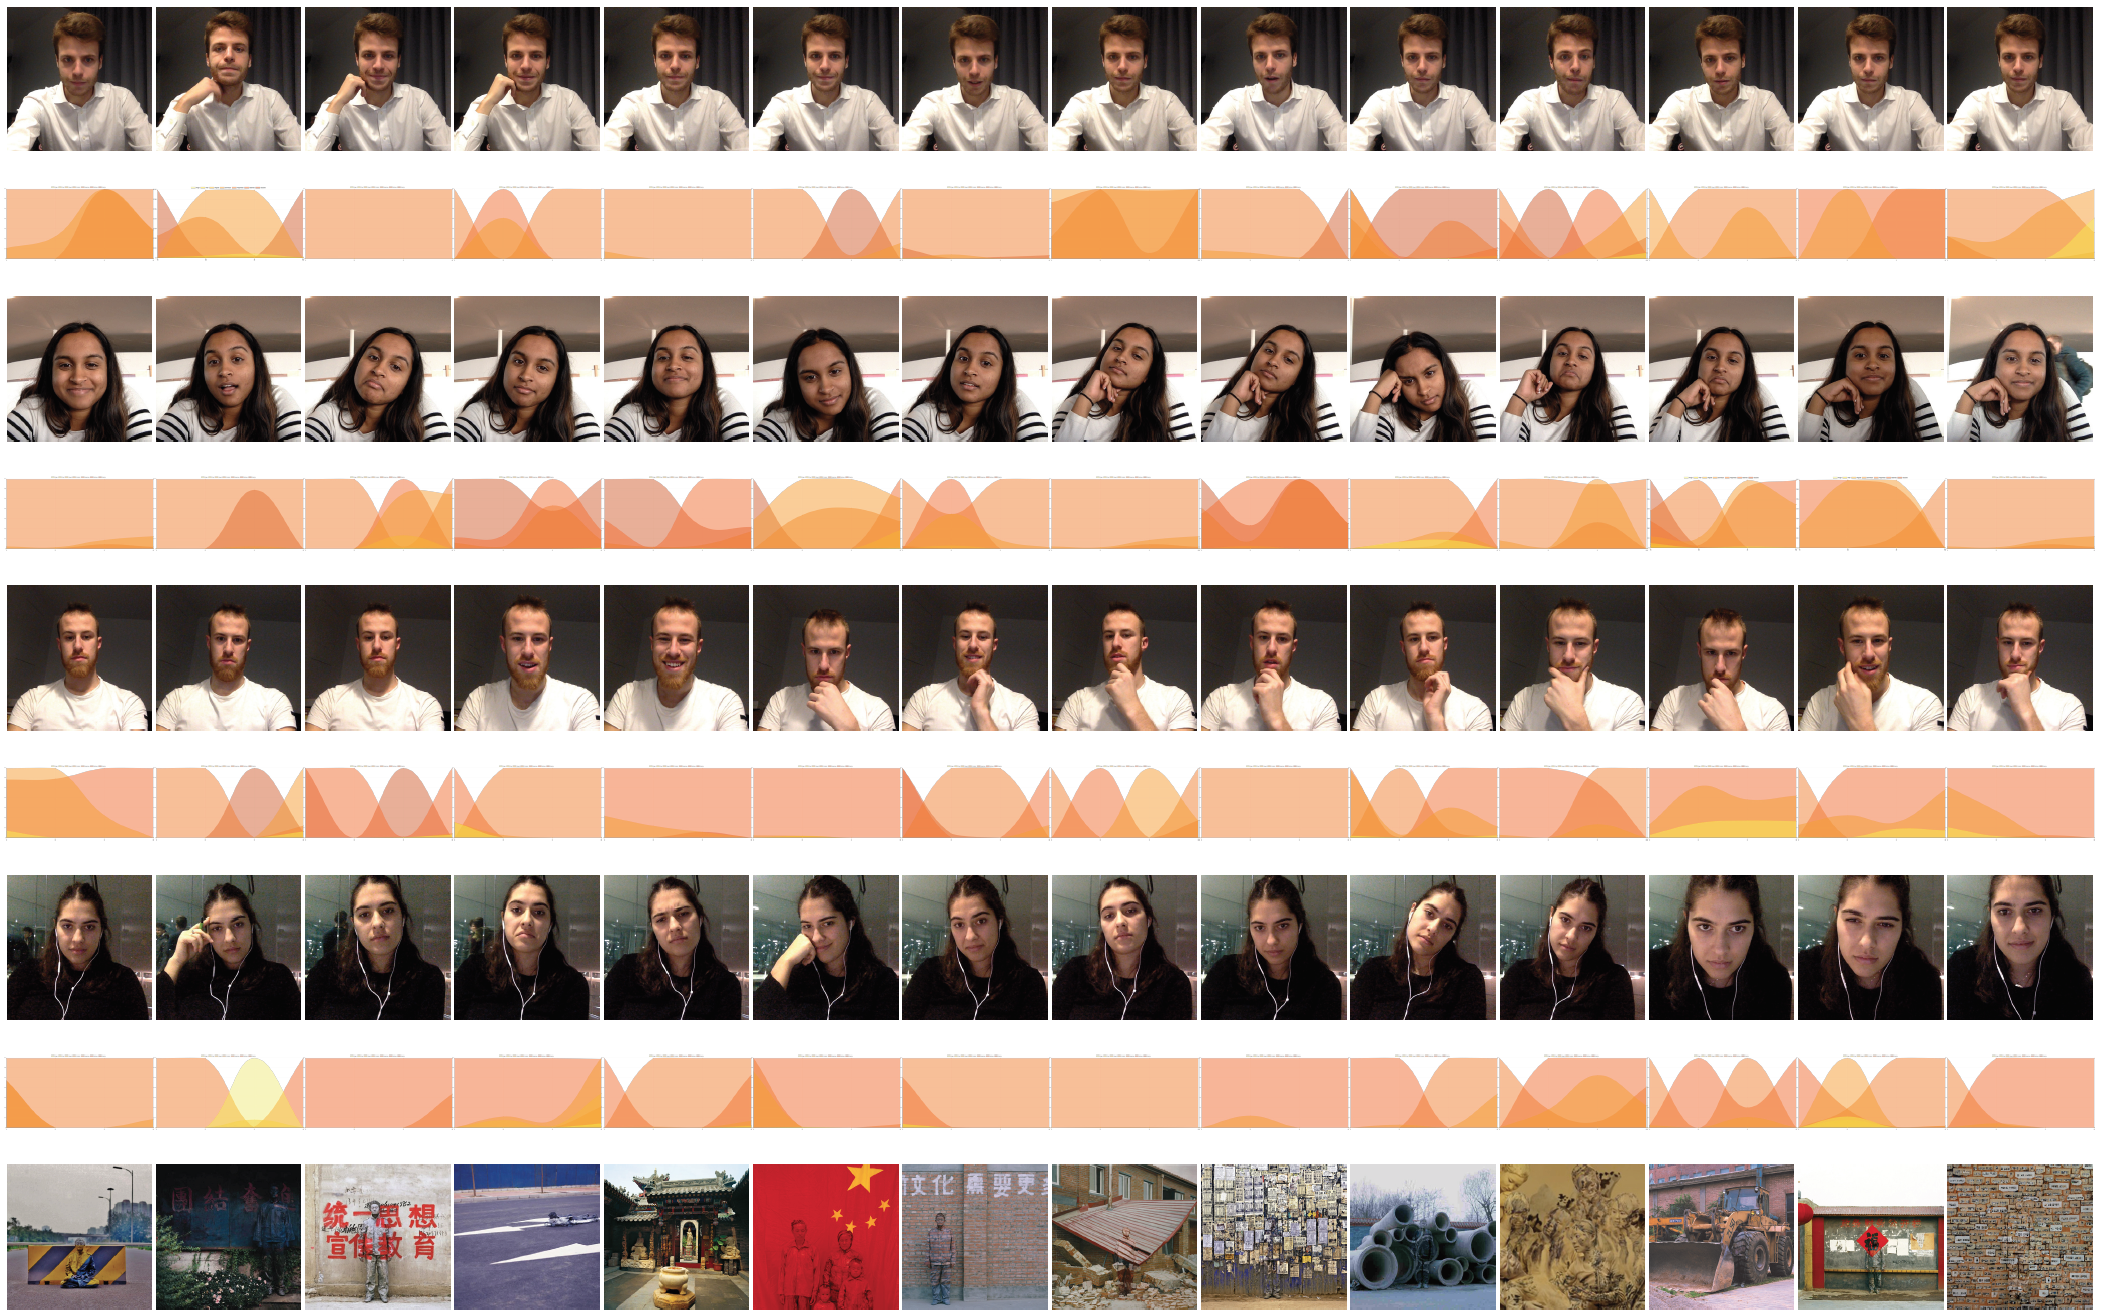
\includegraphics[width=0.49\textwidth]{timeemotion.png}
    \caption{Evolution of emotions during the experiment.}
    \label{fig:time}
\end{figure}
Each recorded picture is then analyzed by the facial recognition software \textit{Face by Microsoft Azure}. Artworks rating is done collecting data through direct observation in a digital museum. By collecting data it was possible to "rate" artworks and people in order to put them in different categories based on the emotions range we aim to analyse. These categories were fundamental to generate our path algorithm as described in section \ref{sec:path}.

\section{Feeling Path} \label{sec:path}
\PARstart{T}{he} idea of the Feeling Path is that one user can get a different way of progressing through the exhibition by balancing the weights of a set of emotions and a time allowed to the visit. The time is in minutes and the emotion vector is just 7 values between 0 and 1 defining the importance of each emotion (disgust, fear, surprise, contempt, anger, sadness and happiness) 0 being the lowest importance and 1 the highest.

In this section we will detail the process of the generation of the Feeling Path and its computation.

\subsection{Path drawing}
We first take a low-resolution image which represents the floor map and define pixels which are reachable and which are not. We can then define an adjacency matrix that will be used to create a graph to be able simulate the navigation in the room. 

At this point, to go from a point to another, we now only need to compute the shortest path using our graph, this will give us the set of pixels crossed in the way. We can then do this for a set of points that we consider to be our path and use the result as control points to draw curves which will illustrate the path. We are using b\'ezier curves to make them smooth and produce a human-like movement. We get the final route by concatenating all the different curves into a single one.
Once we have our path, we can copy it to the fancy illustrated floor plan by re-sizing our curve accordingly.

\begin{figure}[!h]
  \centering
    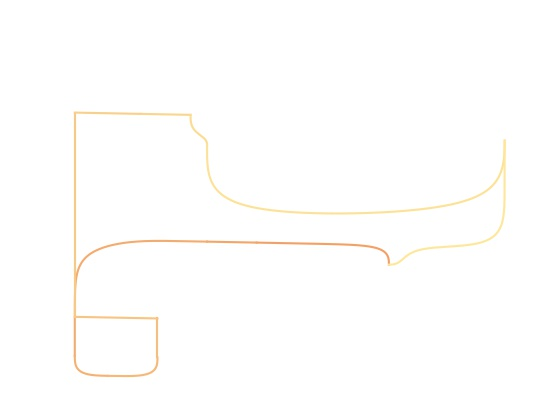
\includegraphics[width=0.35\textwidth]{sPath.jpg}
  \caption{Example of the drawn path.}
  \label{fig:path}
\end{figure}

\subsection{Path computation}
Here we will look into the process which allows to find which pieces of art will be on the path and in which order.

First of all, we need to compute the distance between every pair of artworks and also to include the entry point to this computation. We use the graph representing the floor map created previously to this end. These distances will be used as weights to find the next hop on our path.

We then get the inputs: the emotions vector and the time available from the user. The time will be a threshold to the number of artworks which will be seen by the user, giving us the number of hops.

After that, we begin to construct the path by doing the scalar product of the input vector and the emotion vector of every piece of art to get a similarity score. We then weight these scores by the distance between our actual position and the position of the art piece. The bigger the distance, the lower we are likely to visit it next. Once we decide on our next step, we add the node to the set of visited node so we don't visit it again and set it as our current position. We iterate this way until we reach the wanted number of hops and get back to the exit/entrance point.

This will return our final set of points to visit in order for us to draw the Feeling Path.
\\

\begin{figure}[!h]
  \centering
    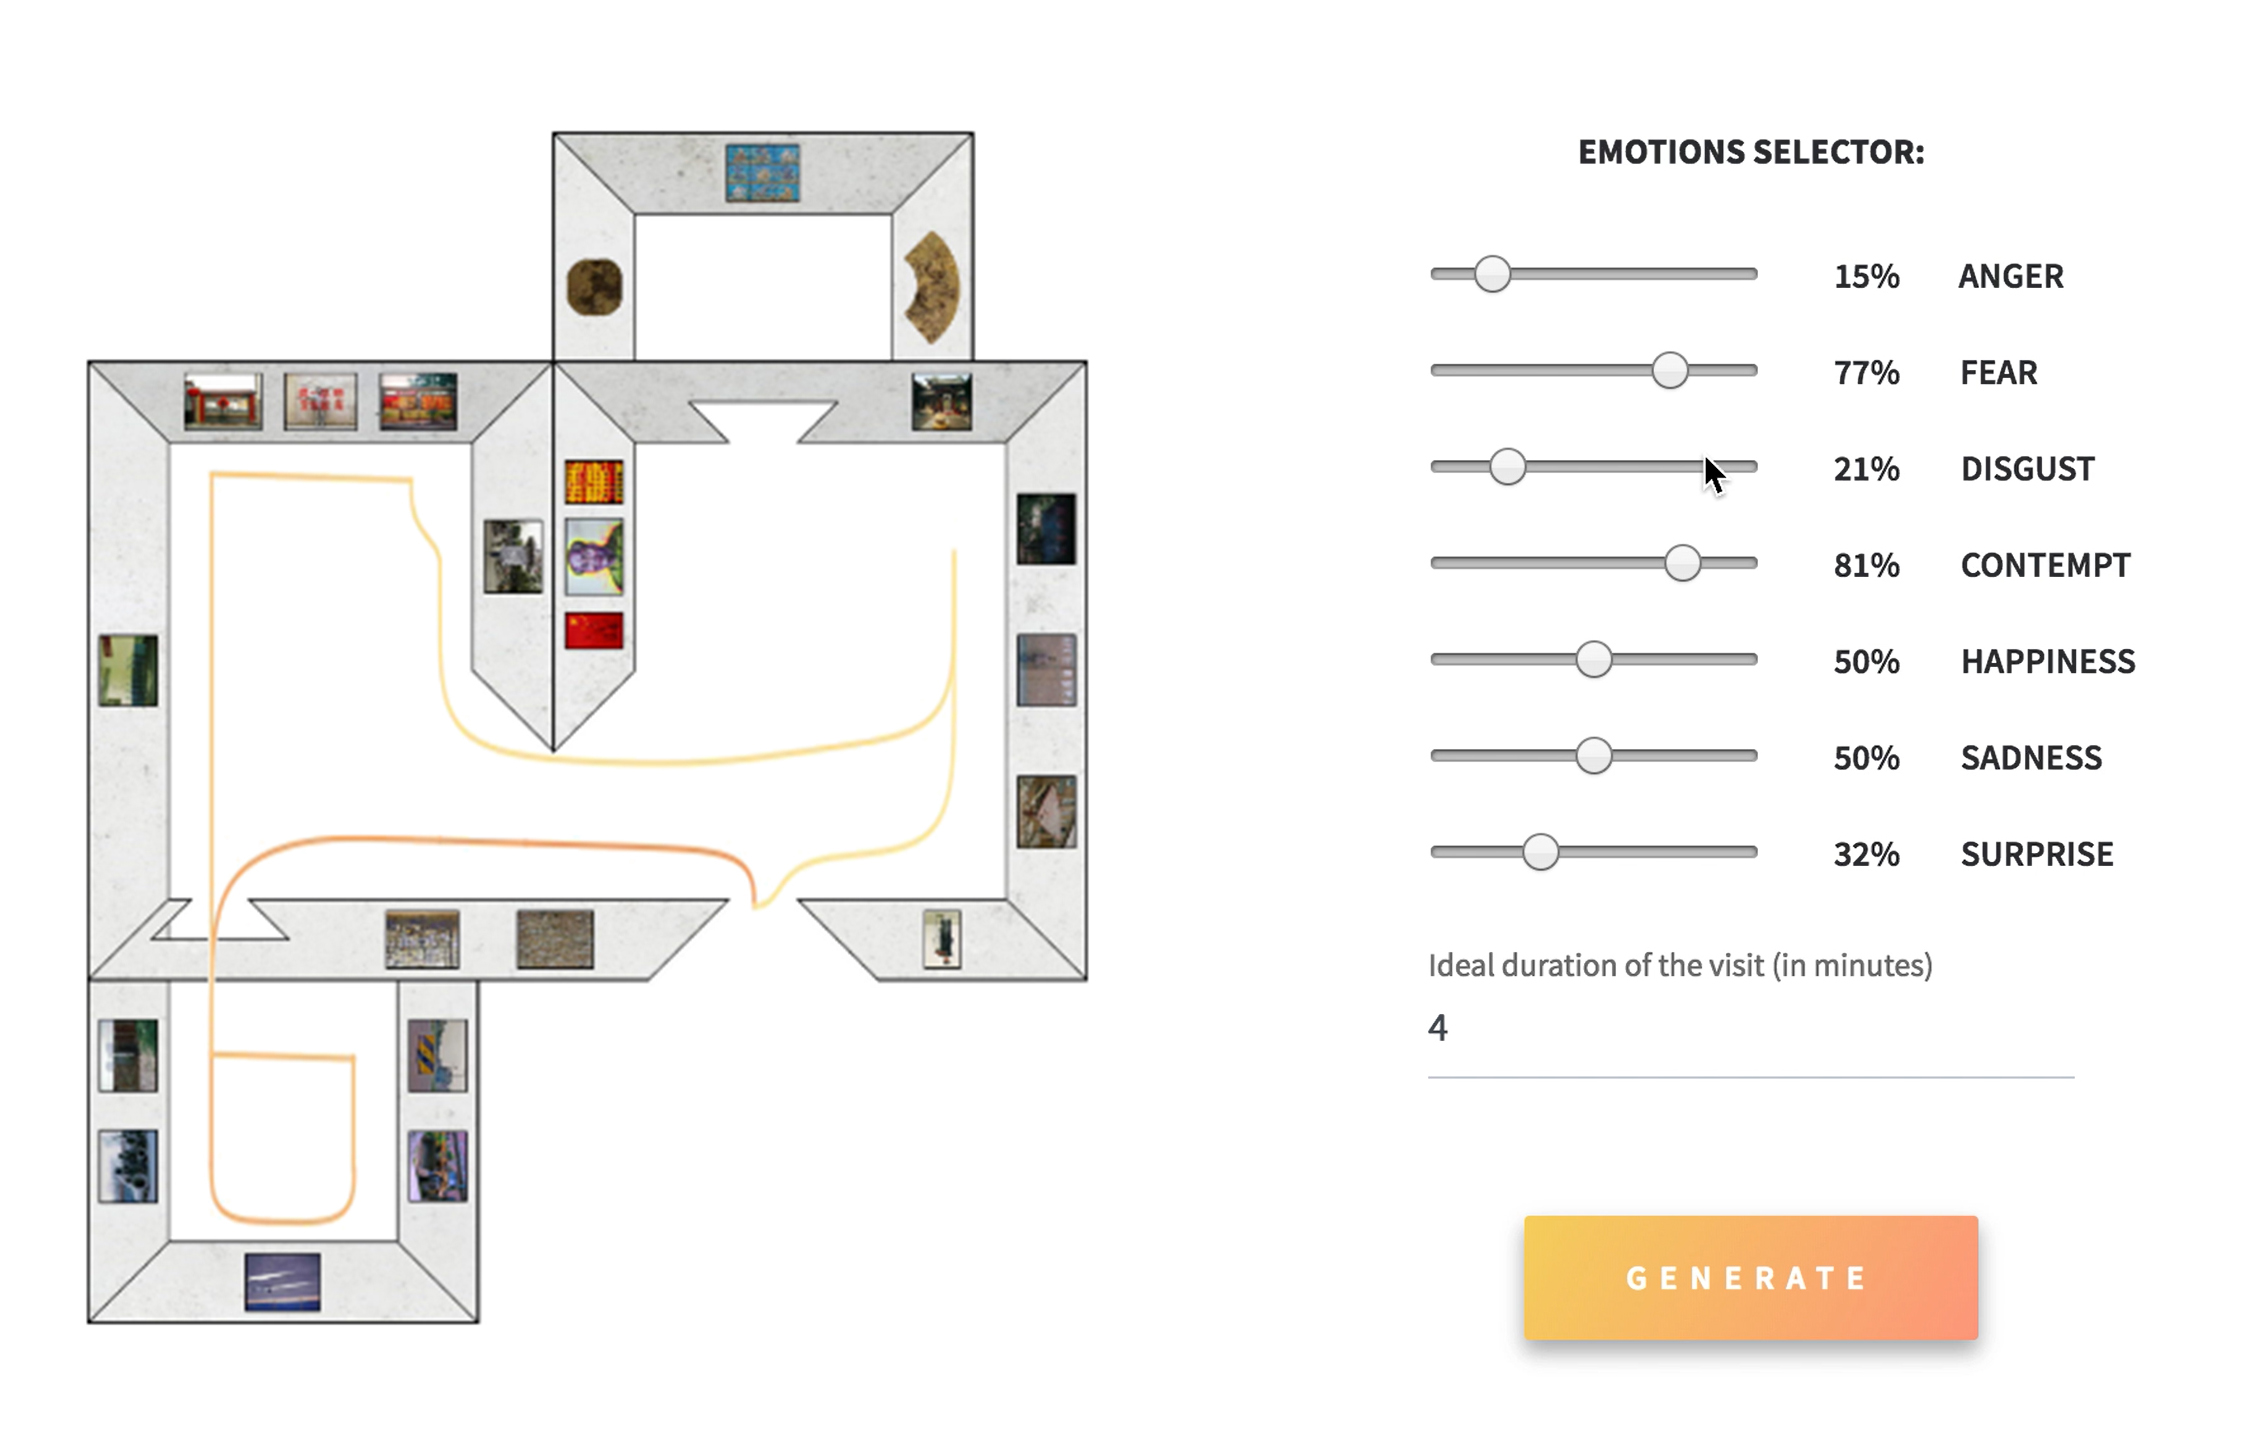
\includegraphics[width=0.38\textwidth]{patherino.jpg}
  \caption{Example of generated Feeling Path.}
  \label{fig:pathToMap}
\end{figure}

\section{Principle Component Analysis: PCA}
\PARstart{O}{nce} the experiment was done and we decided we had gathered enough data from it, we wanted to compare people to the pieces of art such that each person can be face to face with artwork that emotionally resembles them.\\
To this end we used PCA to do dimensionality reduction and being able to represent pictures and people on a 2D plane, having the distance between two points as a metric to the emotional likelihood. As an input to the reduction we use all the emotional vectors from the art pieces and the mean of all persons' reactions during the entire reaction to define them.\\
Finally, we use the PCA functions from scikit-learn Python library to perform our comparison and plot them as below to get visual results.\\


\begin{figure}[h]
    \centering
    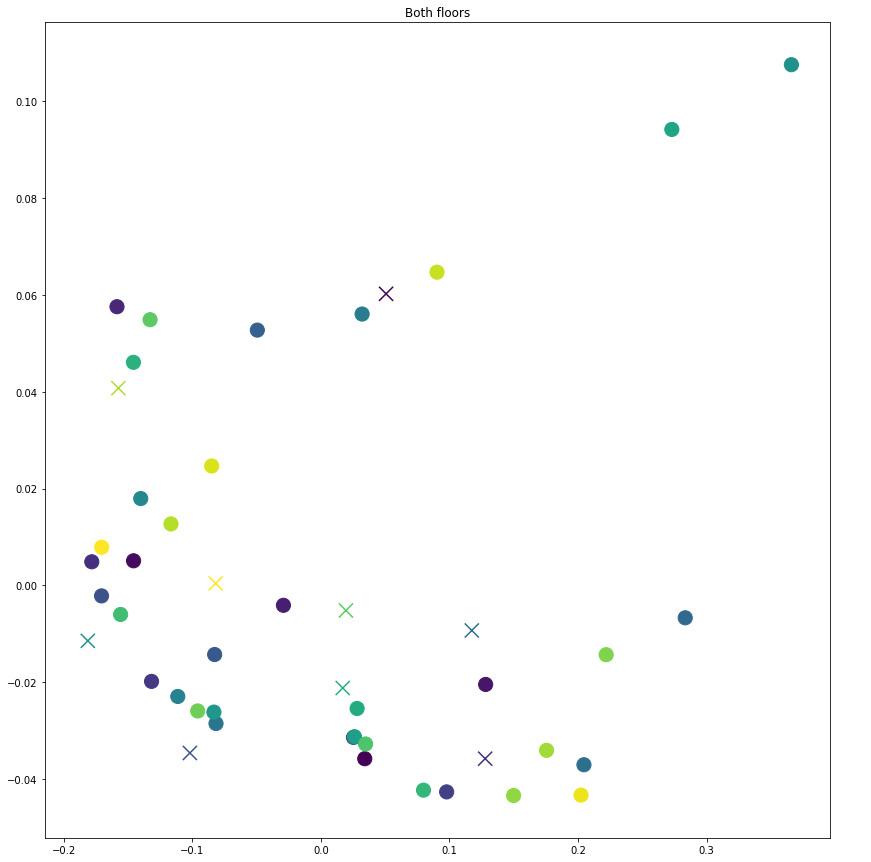
\includegraphics[width=3.8cm]{PCABoth.png}
    \caption{PCA with both floors and people: Circles are the artworks and crosses the different persons.}
    \label{fig:pca}
\end{figure}

As an addition to this, we also found interesting to create two different plots to compare people and pictures from each floor separately. This is because we had two set of people, one who saw the images from both floors and one group who saw the images of the first floor. It hence gives a different vision to the experiment, as we can now show people new artworks directly from their reactions to other exhibits and possibly other museums.

\begin{figure}[!h]
  \centering
  \begin{minipage}[b]{0.24\textwidth}
    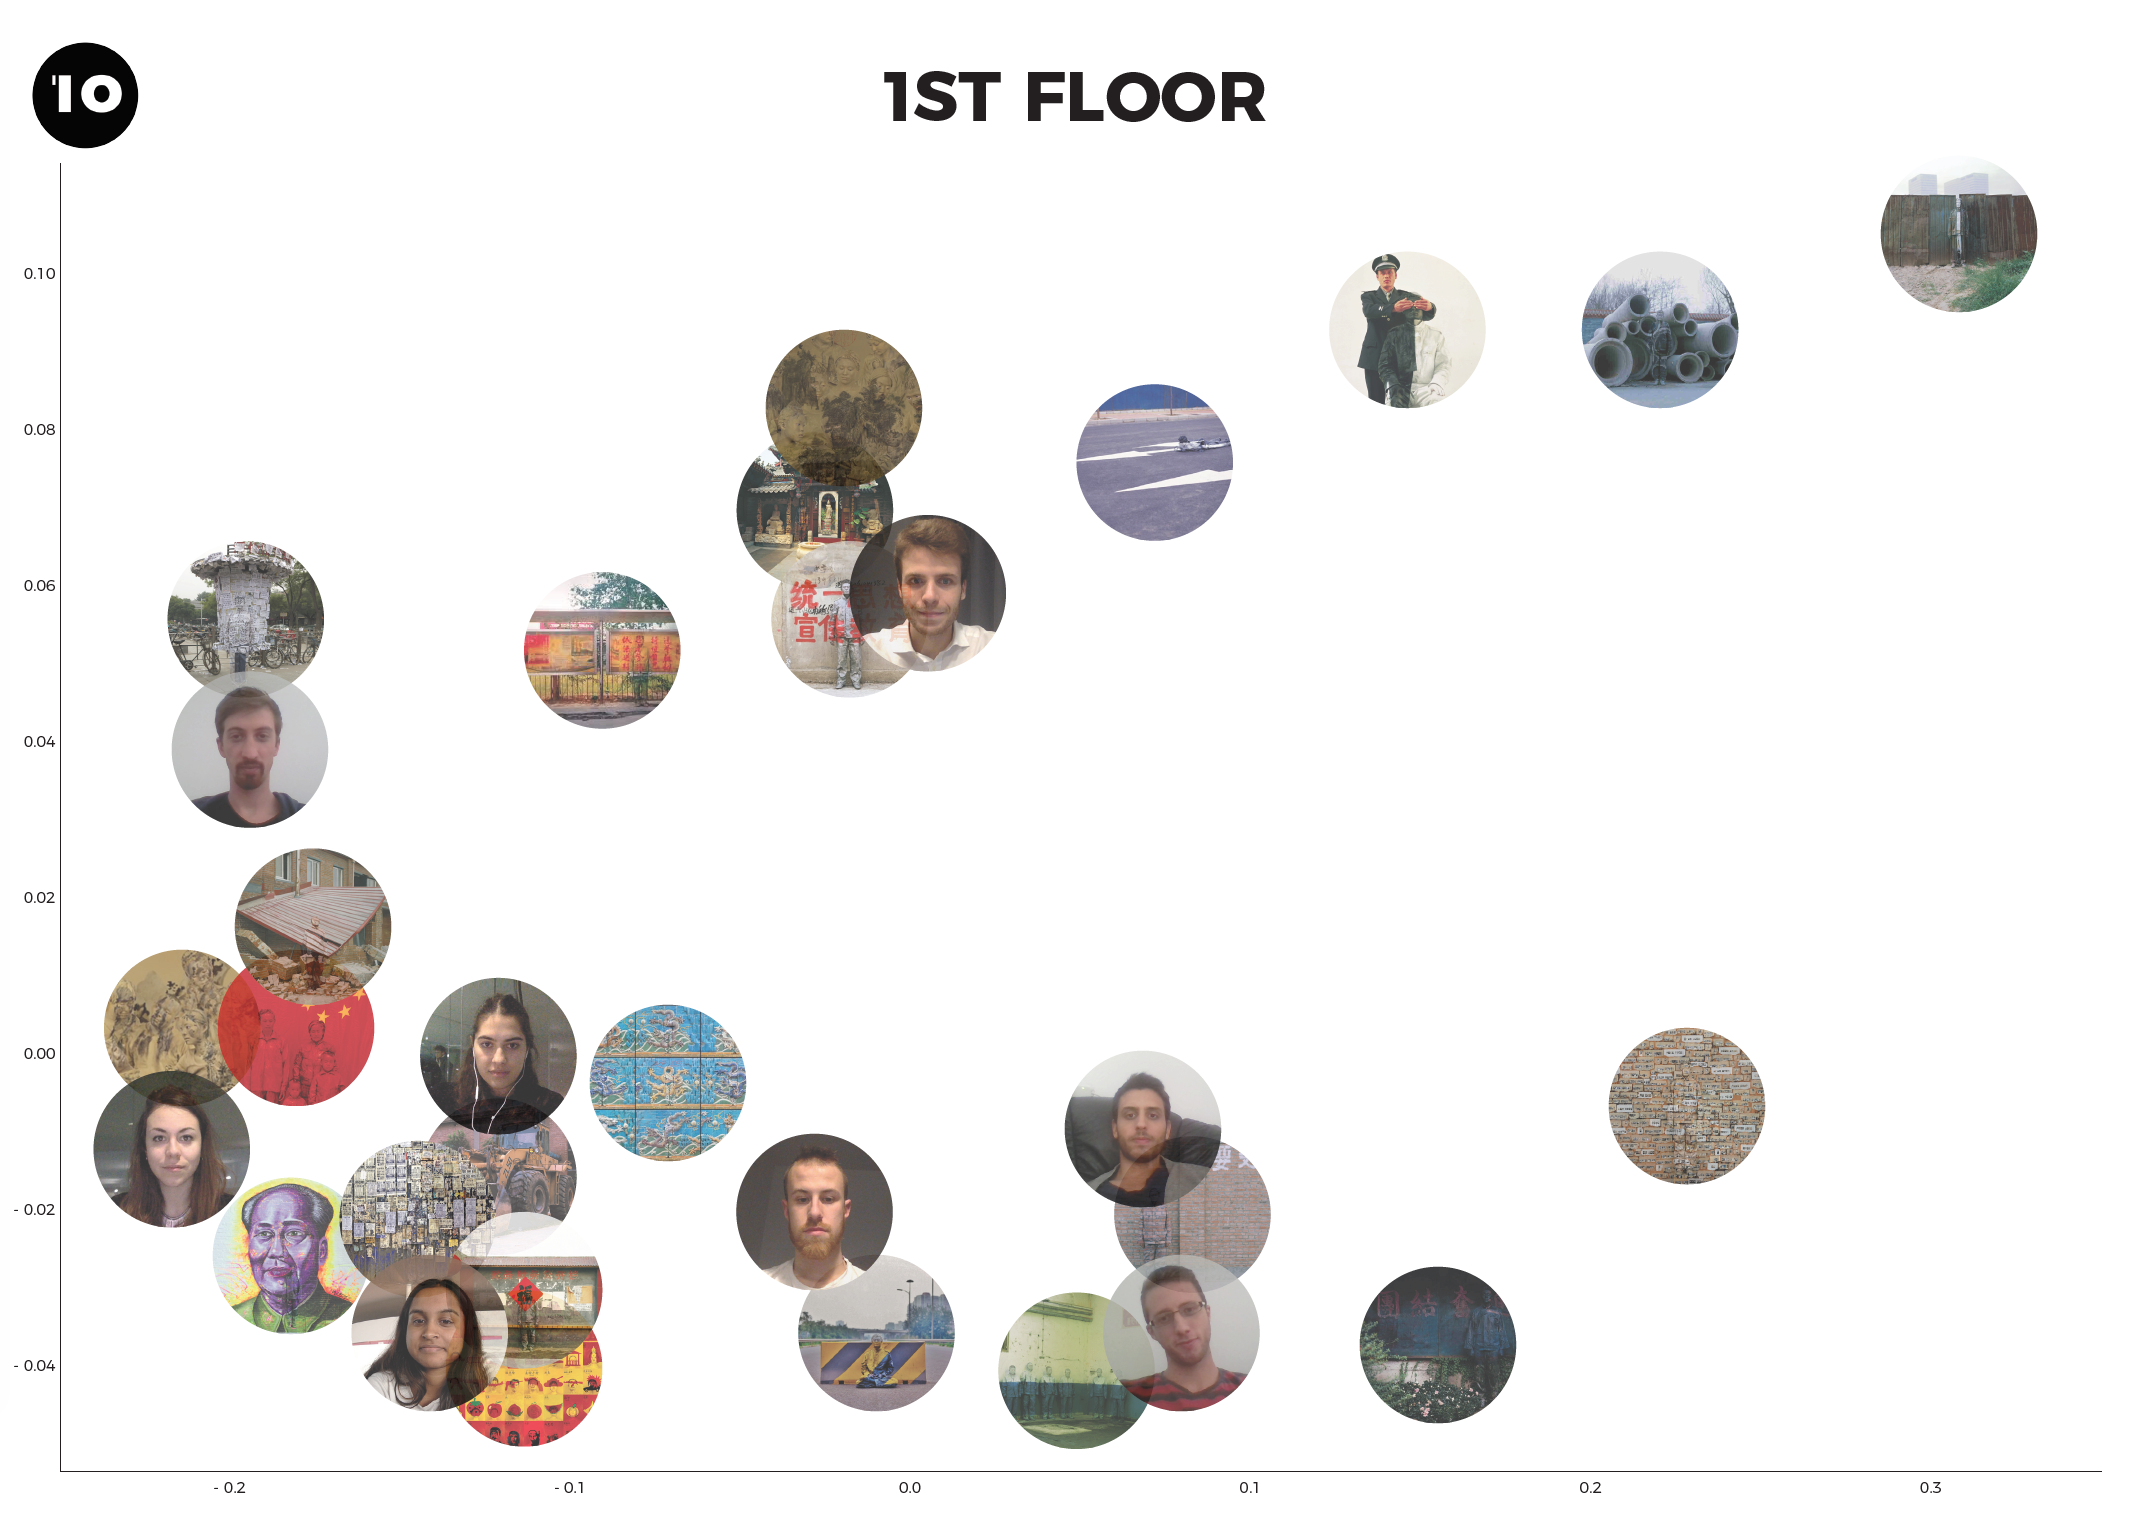
\includegraphics[width=\textwidth]{trainpca.png}
  \end{minipage}
  \hfill
  \begin{minipage}[b]{0.24\textwidth}
    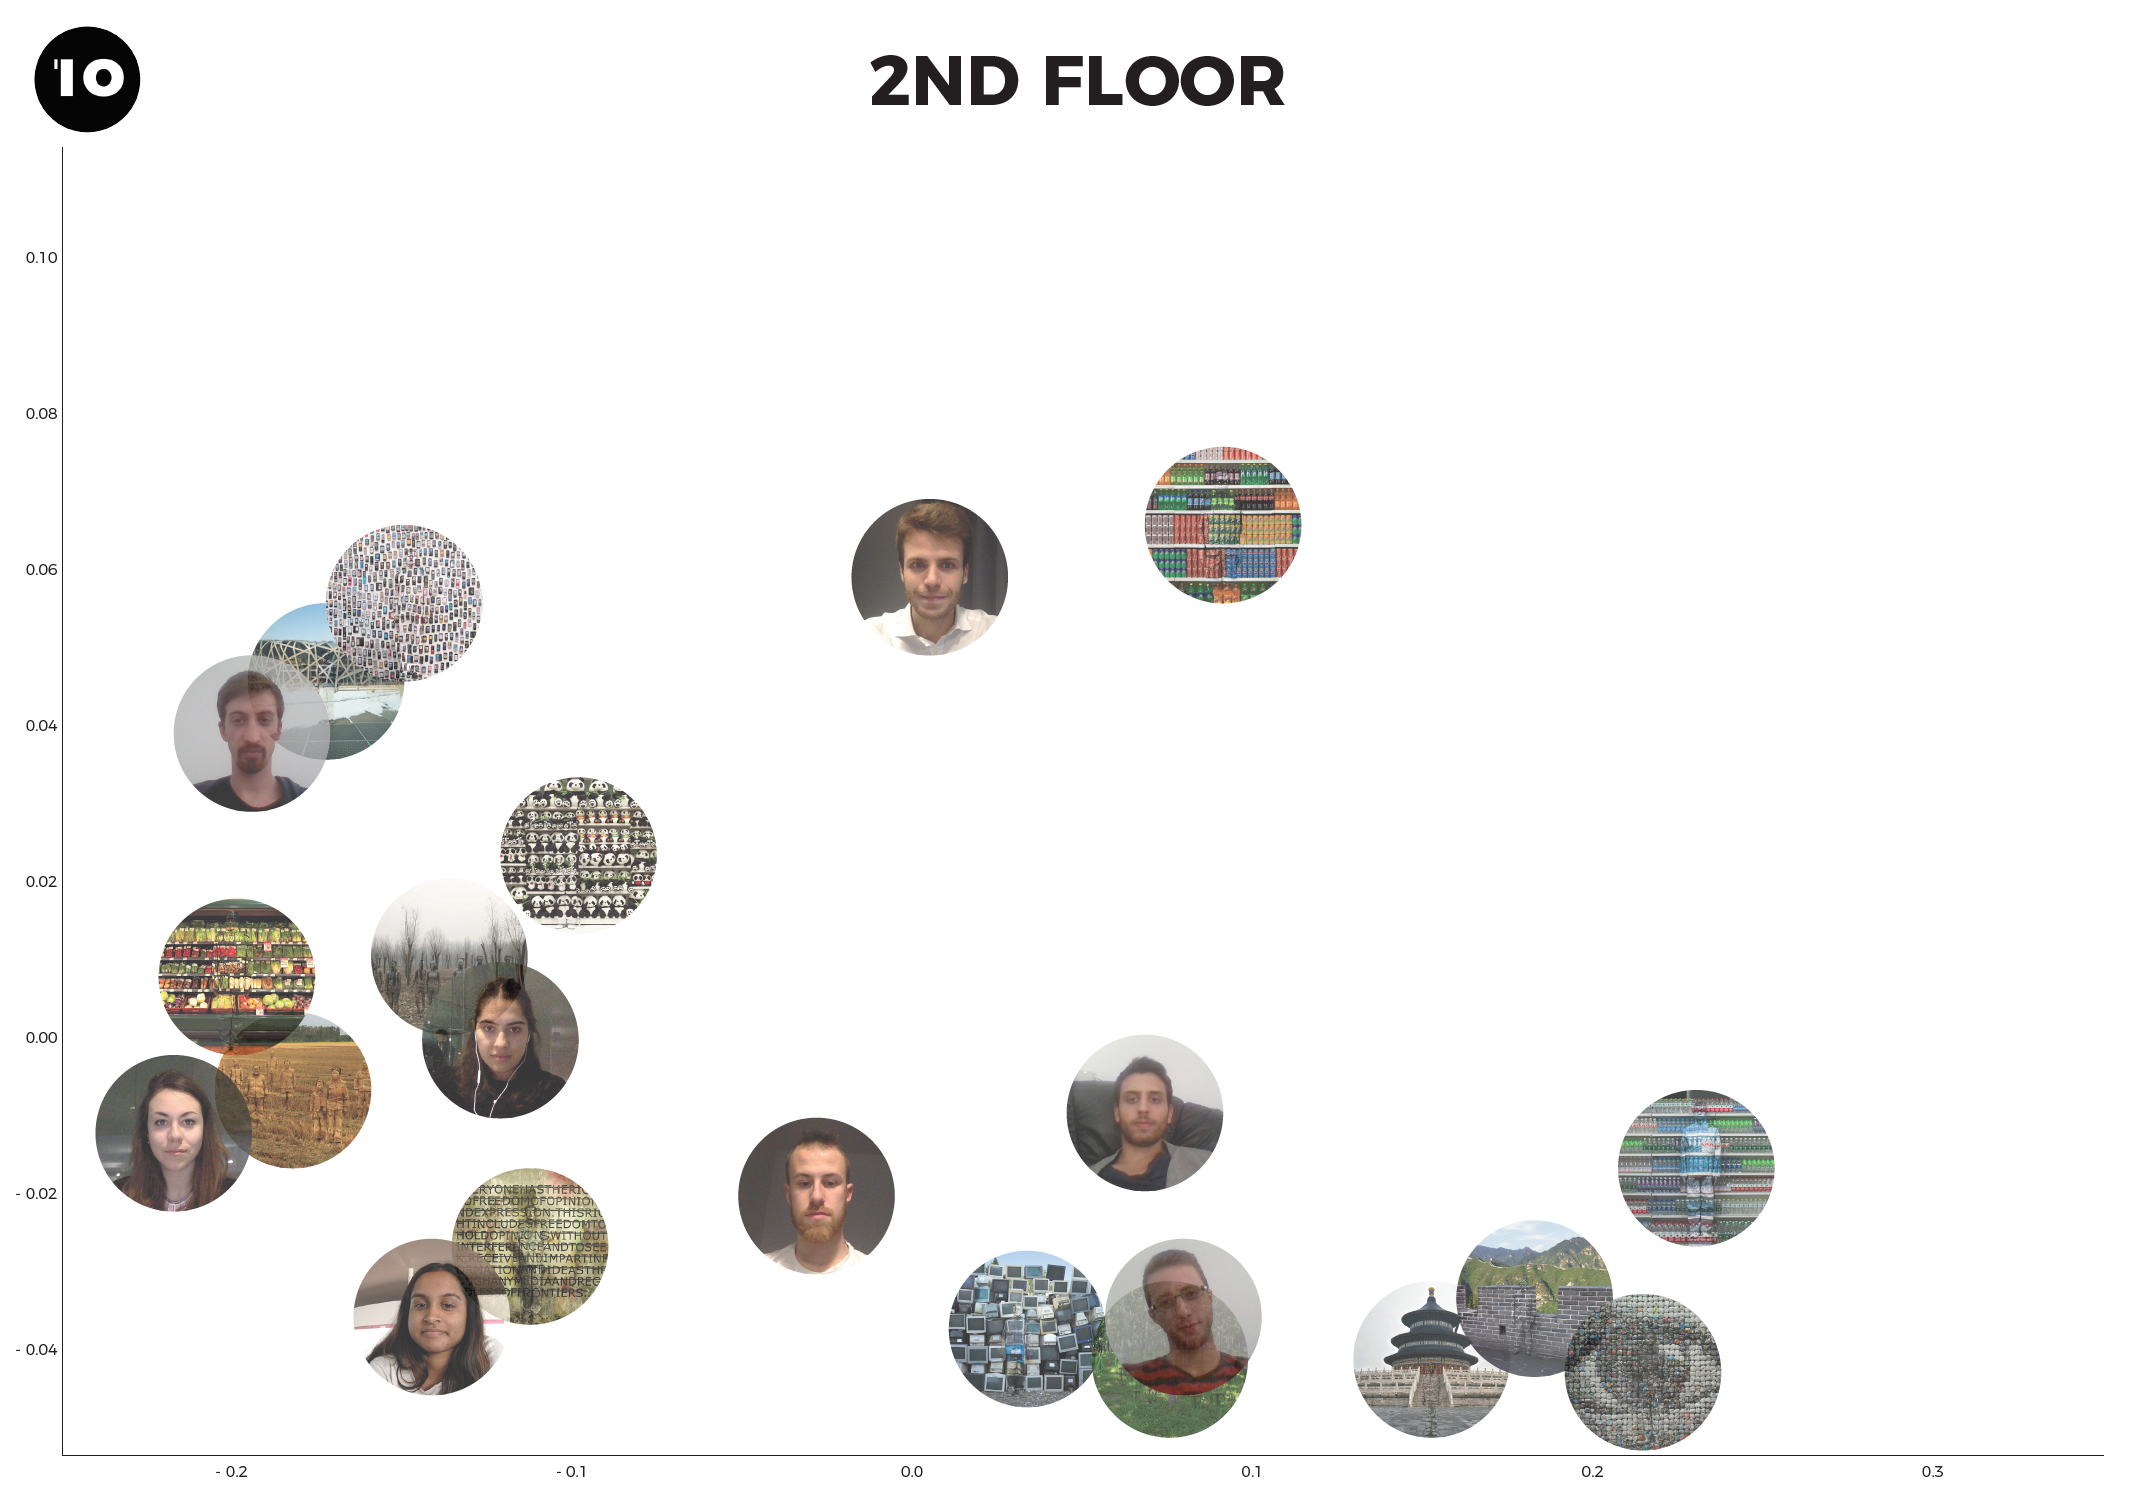
\includegraphics[width=\textwidth]{testpca.png}
  \end{minipage}
  \caption{We have used the first floor to train and the second floor to test.}
  \label{fig:pca-art}
\end{figure}

\section{Web application}
\PARstart{F}{or} the web application we have decided to use the framework Flask\footnote{Flask: \url{http://flask.pocoo.org/}} for the back-end since it is really light and easily expandable. We have factored the application into a set of blueprints \footnote{Blueprint: record operations to execute when registered on an application. Flask associates view functions with blueprints when dispatching requests and generating URLs from one endpoint to another (\url{http://flask.pocoo.org/docs/1.0/blueprints/}).} that allows the instantiation of an application object. To capture the picture during the experiment with the web camera we have used the library \textit{OpenCV}, the experiment starts when the user press the corresponding button on the homepage, every time that a new artwork is showed an \textit{ajax} request is made (see Fig.\ref{fig:experimentim}). The back-end then records 4 pictures for the painting and sends a \textit{GET request} to Microsoft Azure to get the corresponding emotions recorded. 
\begin{figure}[h]
  \centering
  \begin{minipage}[b]{0.24\textwidth}
    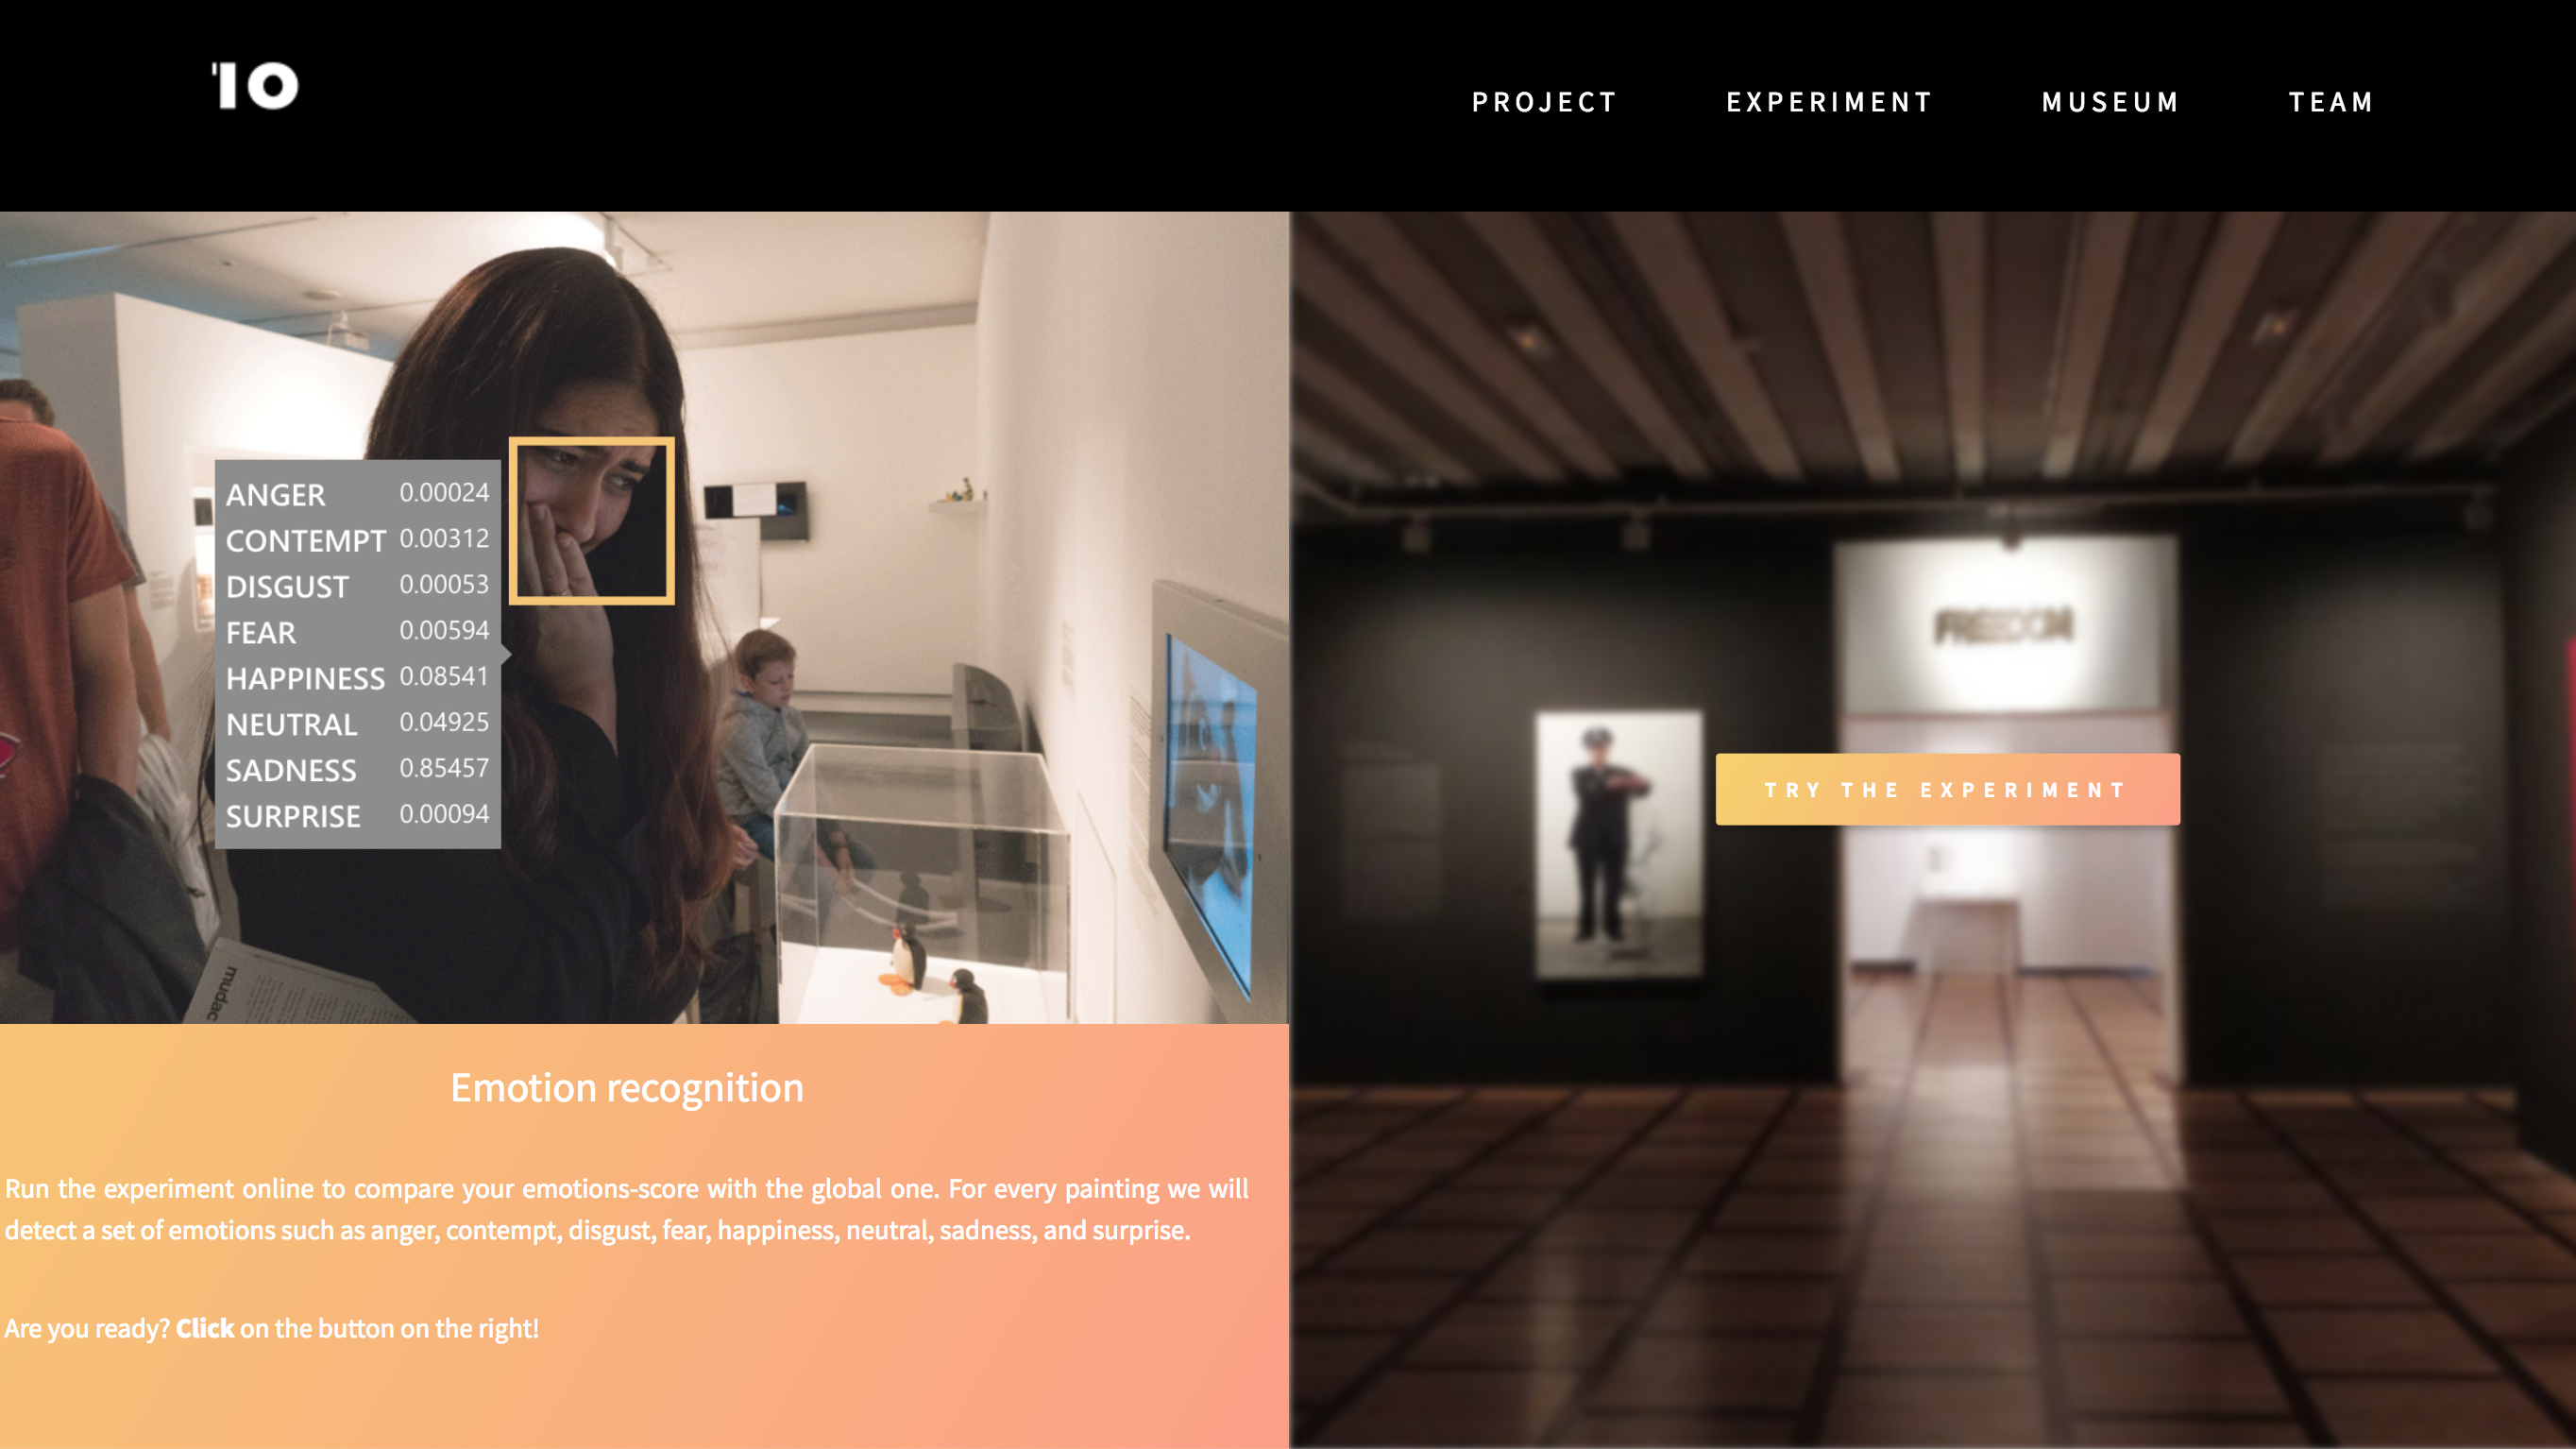
\includegraphics[width=\textwidth]{experiment1.png}
  \end{minipage}
  \hfill
  \begin{minipage}[b]{0.24\textwidth}
    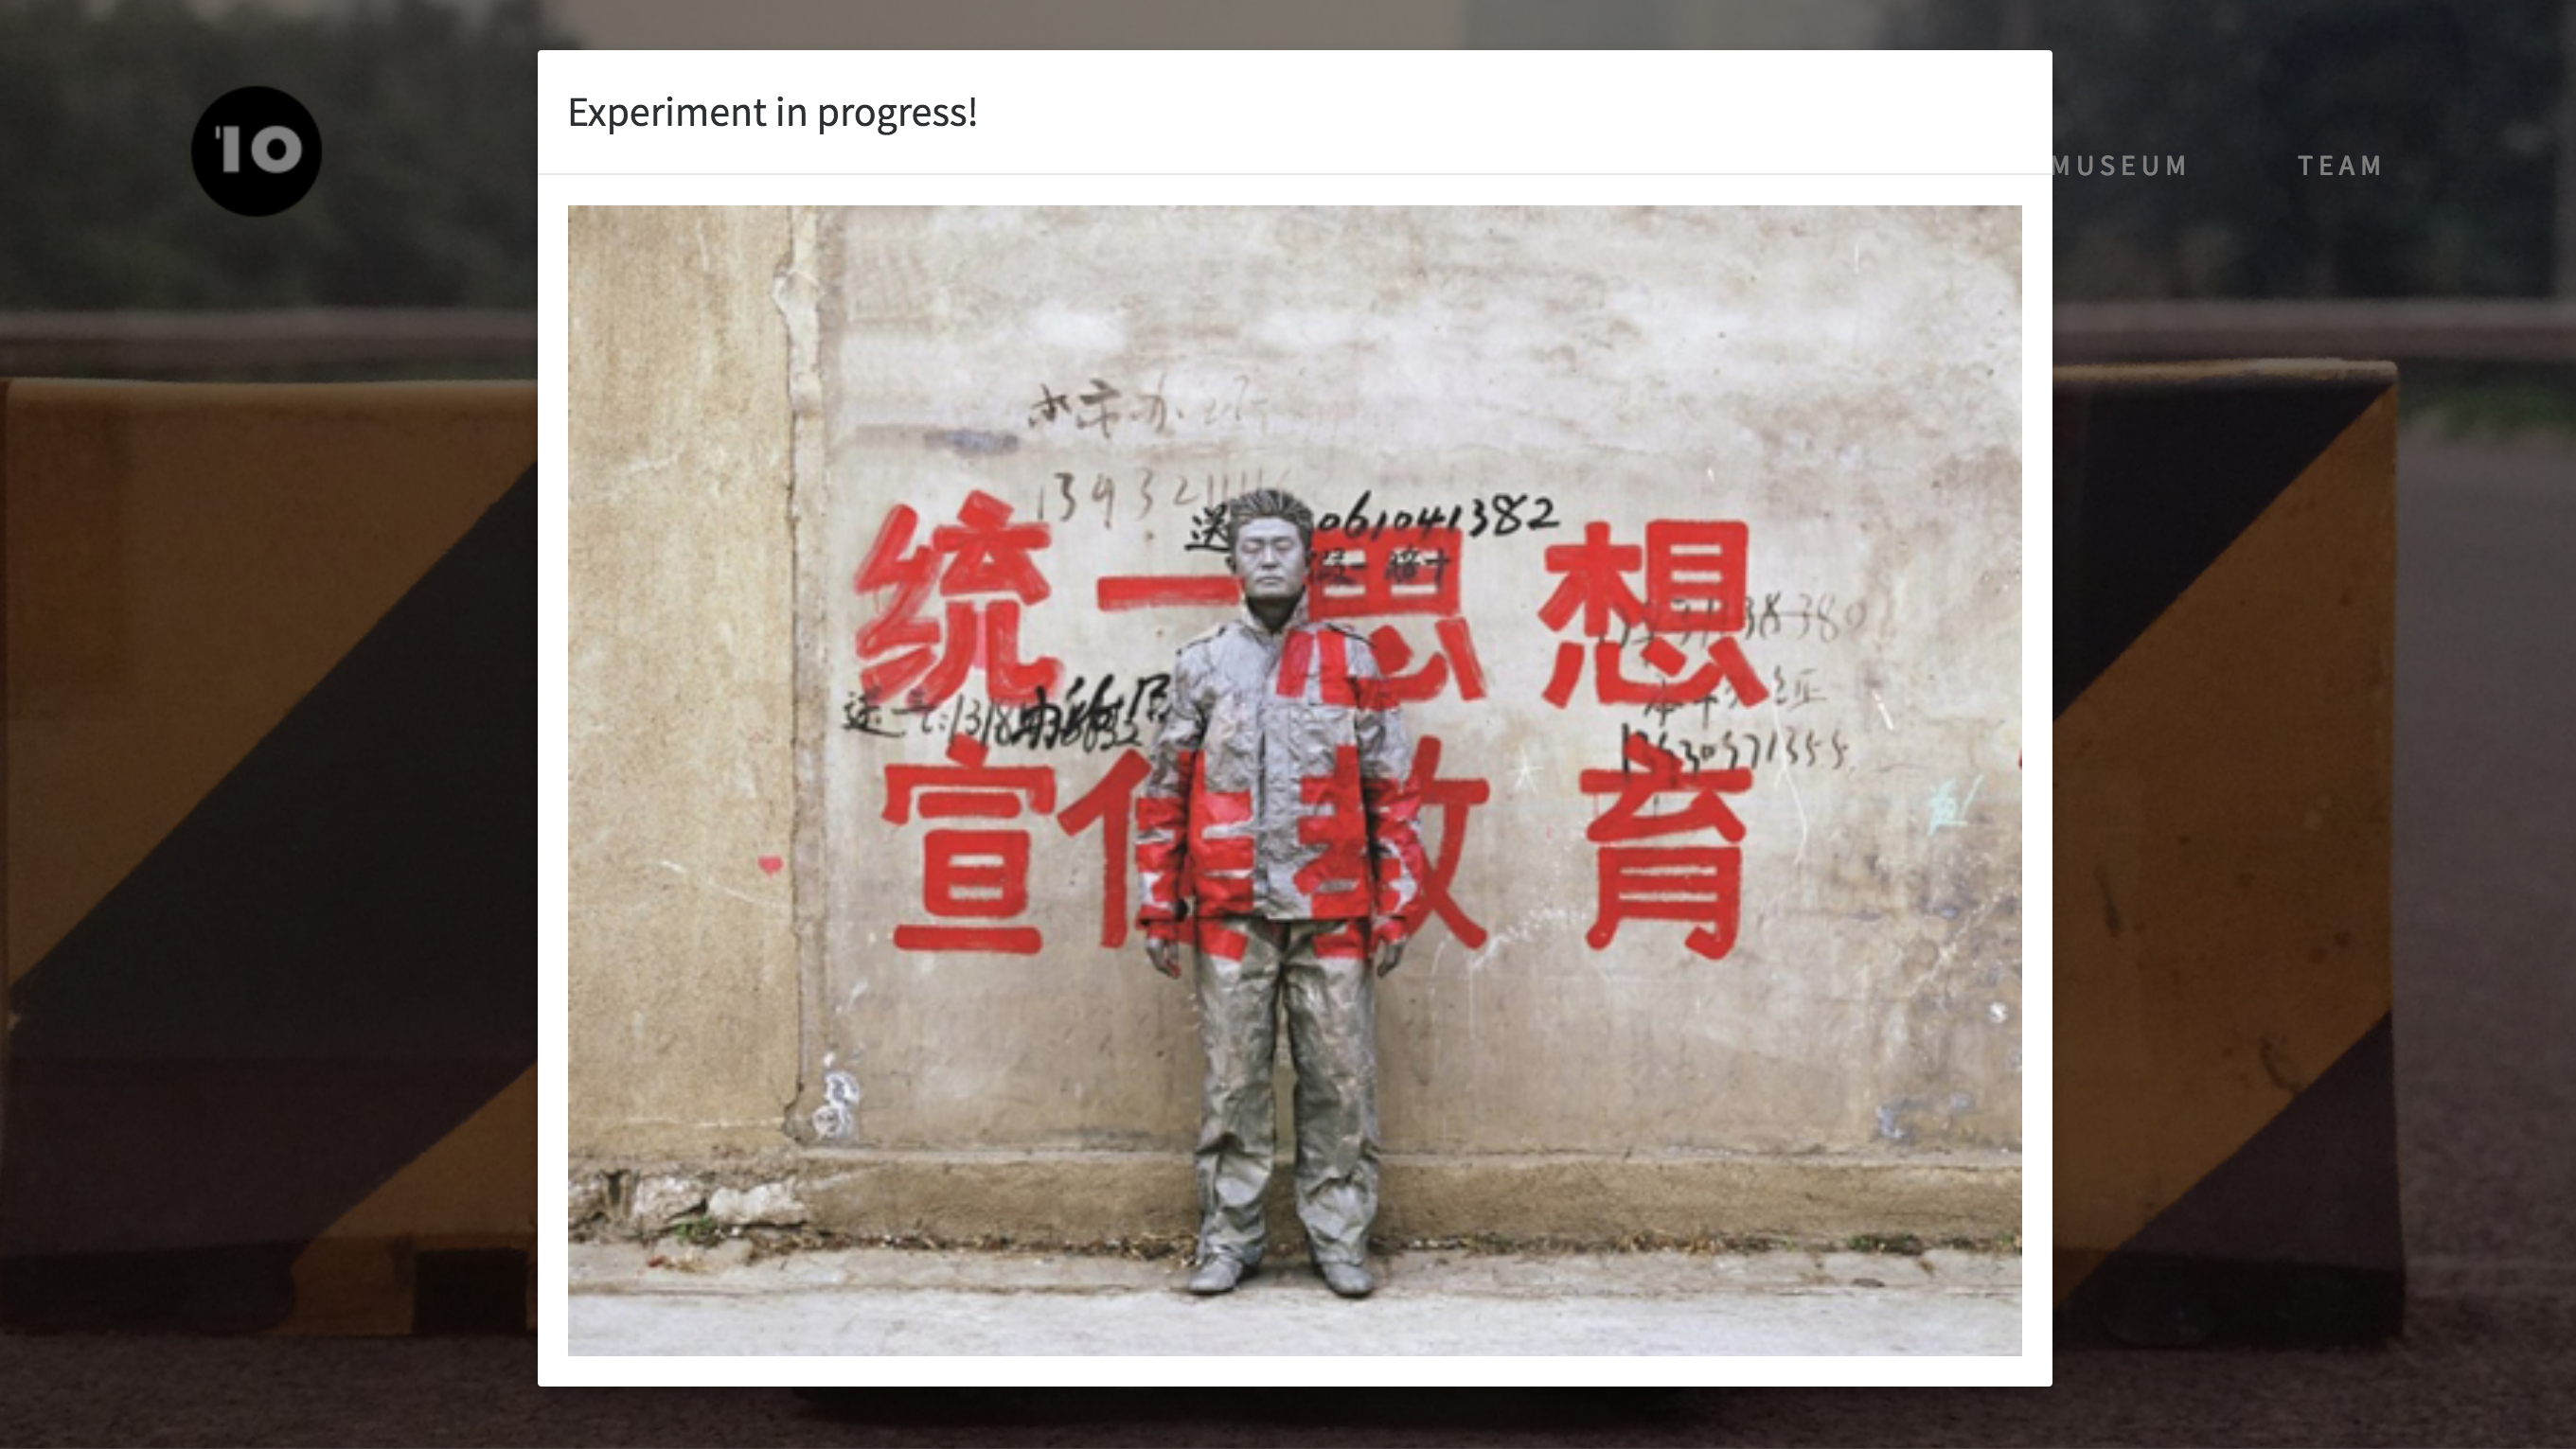
\includegraphics[width=\textwidth]{experiment2.png}
  \end{minipage}
  \caption{Experiment UI}
  \label{fig:experimentim}
\end{figure}
As database we have chosen to use \textit{SQLite3}. At the end of the experiment we insert all the new data into the database. At the end of the experiment a modal containing the results recorded is showed (see Fig.\ref{fig:res}). The user can also look to average data recorded just clicking on the interested painting in the carousel (in the homepage), every time we ask to the back-end to query the corresponding value in order to show an updated chart.
\begin{figure}[h]
    \centering
    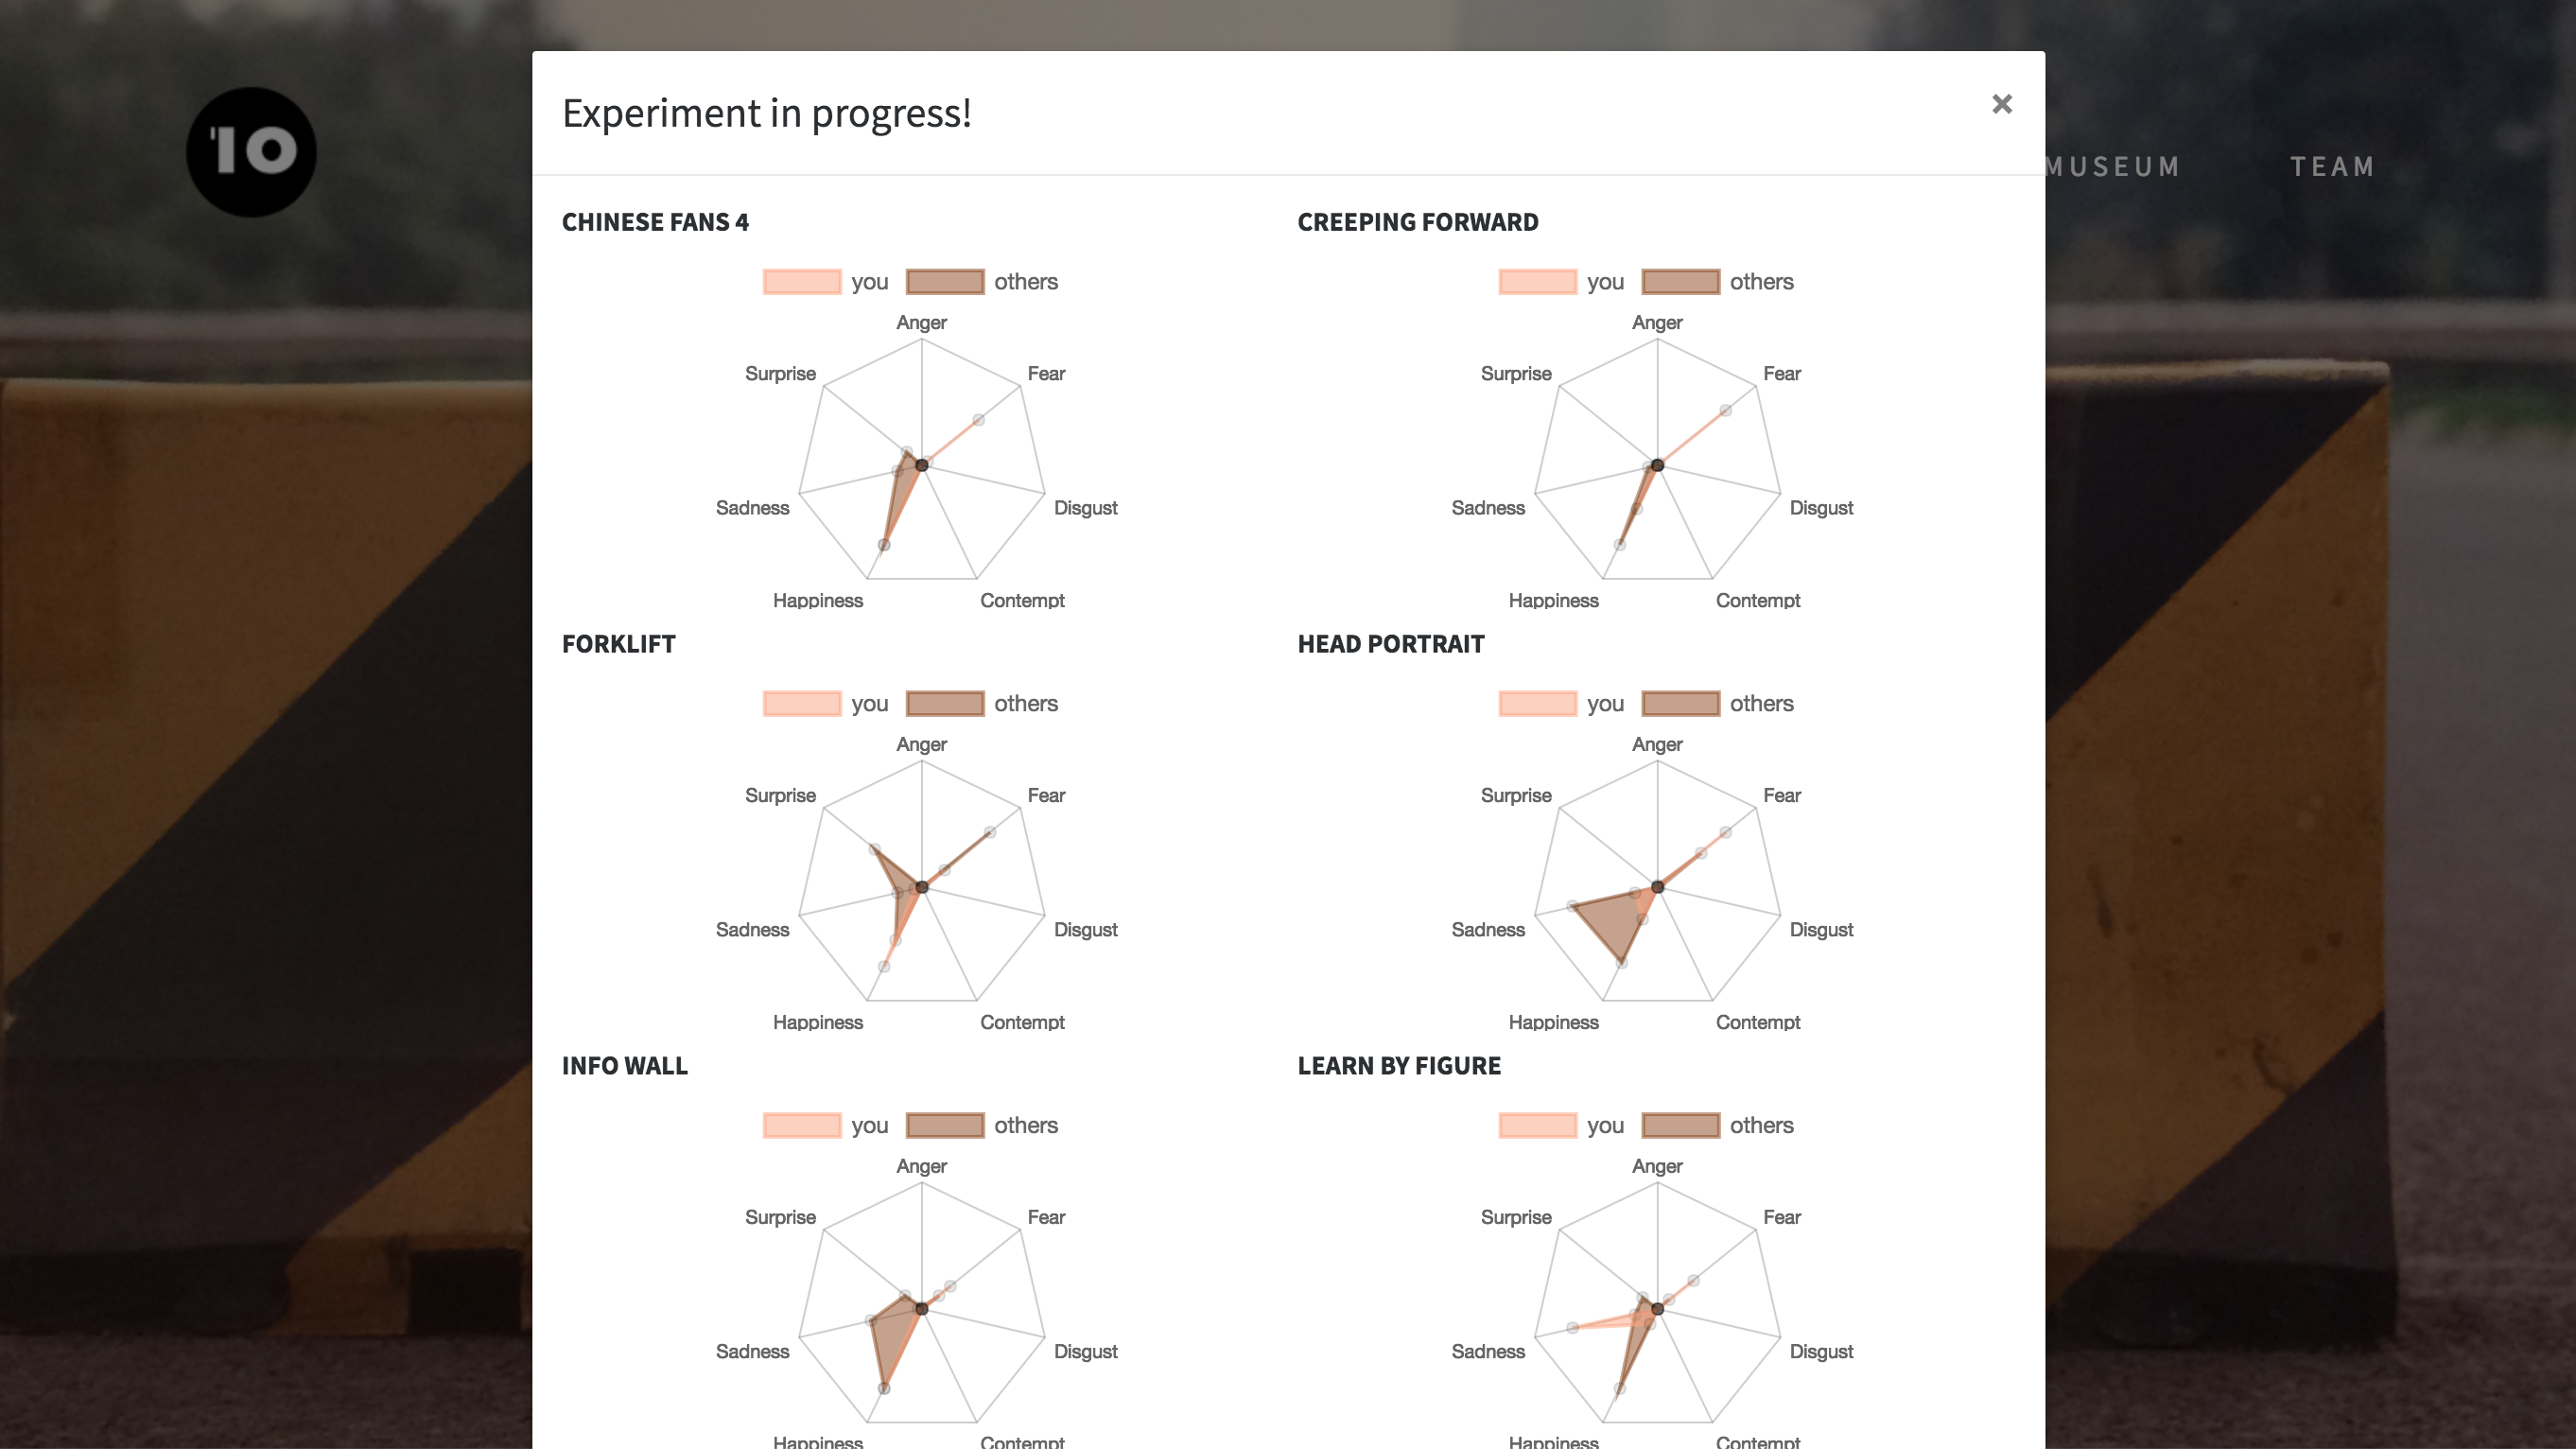
\includegraphics[width=0.49\textwidth]{results.png}
    \caption{Results obtained after having run the experiment.}
    \label{fig:res}
\end{figure}

For the front-end we have used mainly the library \textit{Bootstrap Material Design}\footnote{BootstrapMD: \url{https://mdbootstrap.com/}}. As Javascript library we have used \textit{jQuery}.

To design our web application we have followed the set of rules, guidelines and components proposed by material design.

\section{Conclusion}
% ALL
\PARstart{w}{hat} we aim to do is emphasising this feeling centred attention and let the visitors embrace the essence of the exhibition. This project allowed us to put ourselves in another prospective. We were able to consider artworks not just as a piece of art but to give them somethings that go beyond being material, something that is more abstract: a feeling, an emotion that is intrinsically part of it. As showed in Fig. (\ref{fig:pca-art}) we can notice that some people almost full overlay with certain artworks, that means that are emotionally similar. The website grants people interested in the project to look at results that we have collected during the experiment (see Fig. \ref{fig:charttime}).
\begin{figure}[!h]
  \centering
  \begin{minipage}[b]{0.24\textwidth}
    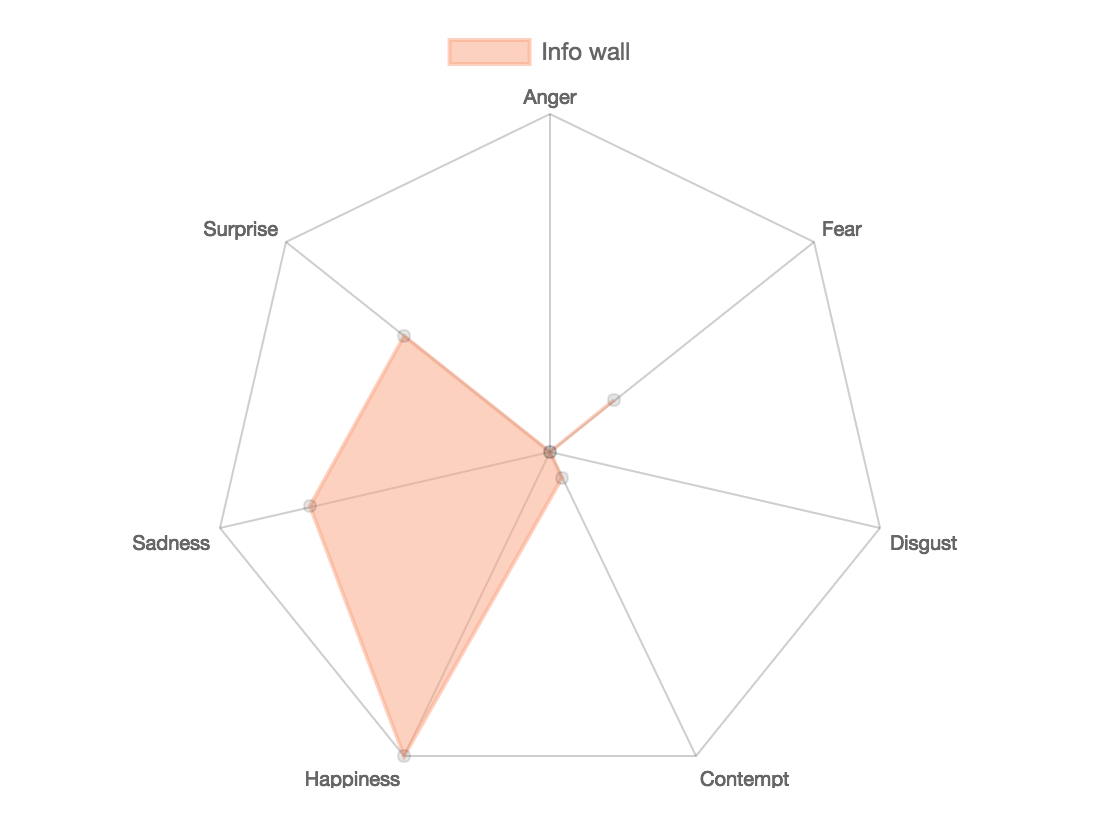
\includegraphics[width=\textwidth]{chart.png}
  \end{minipage}
  \hfill
  \begin{minipage}[b]{0.24\textwidth}
    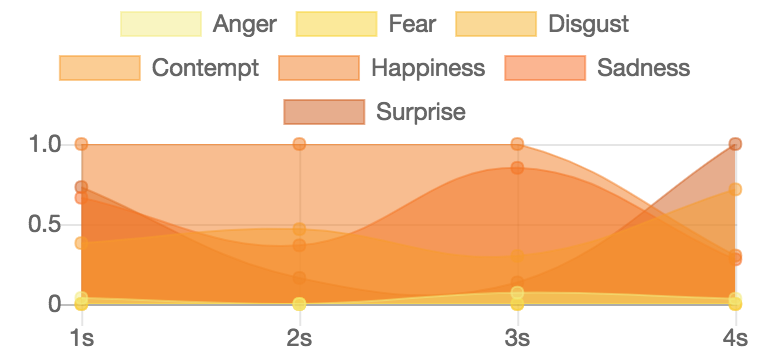
\includegraphics[width=\textwidth]{emot.png}
  \end{minipage}
  \caption{Result of the emotion obtained for the artwork \textit{Info wall}. On the left: emotions average distribution, on the right: evolution of the emotions during 6 seconds.}
  \label{fig:charttime}
\end{figure}

\end{document}